\documentclass{article}
\usepackage[margin=1in]{geometry}  % Helps with proper margins
\usepackage{amsmath}               % For mathematical symbols and align environment
\usepackage{graphicx}              % For including images
\usepackage{amssymb}               % For additional symbols

\begin{document}

\section*{A10}

\subsection*{(a)}
The value of \( n \) is calculated to be 40000.

\subsection*{(b)}
As \( k \) increases, the empirical CDF of \( Y^{(k)} \) becomes closer to the CDF of the standard normal distribution.

\begin{figure}
    \centering
    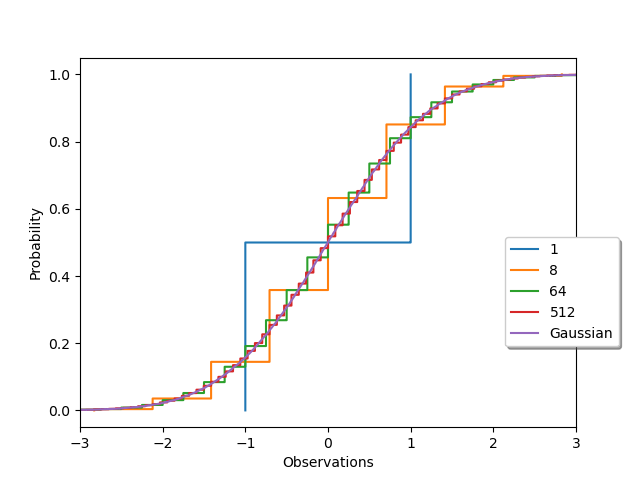
\includegraphics[width=0.5\linewidth]{C:/Users/admin/Downloads/ML/hw0/hw0-tex/plot1.png}
    \caption{Empirical CDF of \( Y^{(k)} \)}
    \label{fig:empirical-cdf}
\end{figure}

\end{document}